% For tracking purposes - this is V2.0 - May 2012
%f=PAR; latex $f.tex; bibtex $f; latex $f.tex; latex $f.tex; dvips -t letter $f; ps2pdf $f.ps; evince $f.pdf
% --- Leon: Packages ---
\documentclass{sig-alternate}

%\documentclass{acm_proc_article-sp}

\usepackage{epsfig}
\usepackage{eqparbox}
\usepackage{url}
\usepackage{verbatim}
\usepackage[utf8]{inputenc}
\usepackage[T1]{fontenc}
\usepackage{microtype}
%\usepackage[nocompress]{cite}
\hyphenation{op-tical net-works semi-conduc-tor}
\usepackage{balance}
%\usepackage[cmex10]{amsmath}
%\usepackage{amssymb,amsfonts,textcomp}
%\usepackage{multicol}
%\usepackage{array}
% --- End of Packages ---

\begin{document}
%
% --- Author Metadata here ---
\conferenceinfo{ICSE}{'14, May 31 - June 7, 2014, Hyderabad, India}
\CopyrightYear{14}
\crdata{978-1-4503-2768-8/14/05}
%\CopyrightYear{2007} % Allows default copyright year (20XX) to be over-ridden - IF NEED BE.
%\crdata{0-12345-67-8/90/01}  % Allows default copyright data (0-89791-88-6/97/05) to be over-ridden - IF NEED BE.
% --- End of Author Metadata ---

\title{Product Assignment Recommender}

\numberofauthors{2}
\author{
           Jialiang Xie$^{1,2}$, Qimu Zheng$^{1,2}$, Minghui Zhou$^{1,2}$\titlenote{Corresponding author.}, Audris Mockus$^3$\\
       \affaddr{$^1$School of Electronics Engineering and Computer Science, Peking University}\\
       \affaddr{$^2$Key Laboratory of High Confidence Software Technologies, MoE}\\
       \affaddr{$^3$Avaya Labs Research, Basking Ridge, NJ, USA}\\ \\
       \eaddfnt{leonxj@gmail.com, zheng.qm@163.com, zhmh@pku.edu.cn, audris@avaya.com}
 }
\date{March 14, 2014}

\hyphenation{ITS}
\clubpenalty=10000
\widowpenalty=10000
\displaywidowpenalty=10000

\maketitle
\begin{abstract}
  Effectiveness of software development process depends on the
  accuracy of data in supporting tools. In particular, a customer
  issue assigned to a wrong product team takes much longer to
  resolve (negatively affecting user-perceived quality) and wastes
  developer effort. In Open Source Software (OSS) and in commercial projects
  values in issue-tracking systems (ITS) or Customer
  Relationship Management (CRM) systems are often assigned by
  non-developers for whom the assignment task is difficult.
  We propose PAR (Product Assignment Recommender) to
  estimate the odds that a value in the ITS is
  incorrect. PAR learns from the past activities in ITS and performs
  prediction using a logistic regression model. Our demonstrations show how
  PAR helps developers to focus on fixing real problems, and how it can
  be used to improve data accuracy in ITS by crowd-sourcing
  non-developers to verify and correct low-accuracy data.  \url{http://youtu.be/IuykbzSTj8s}
\end{abstract}
\vspace{-.3cm}
\category{D.2.6}{Software Engineering}{Metrics}
\vspace{-.2cm}
\terms{Measurement}
\vspace{-.2cm}
\keywords{Product Assignment, Quality Monitoring, Data Quality}

%\vspace{-.275cm}
\section{Introduction}
Many software activities depend on the accuracy of data recorded in
the development support tools. For example, ITS supports
tracking and resolving issues. In particular, the values of various
fields in ITS determine the workflow for an issue. In commercial CRM
systems, as well as in open source ITS, the issue
 reporter or triager determines the product at fault.
Developer time is expensive or limited,  so the triage tasks
(filtering incoming issues to determine if they are valid,
completing necessary information, and determining the
location/product~\cite{XZM13}) for user-reported issues are usually done by
non-developer volunteers in OSS or by service technicians in commercial
projects.  For example, in Mozilla, non-developer volunteers helped
to assign 29\% of issues, while in commercial projects
customer-reported issues are typically first triaged by the support
staff of non-developers~\cite{XZM13}.

Determining the product at fault is typically not an easy task, especially for
non-developers~\cite{XZM13}, leading to a substantial fraction of
incorrect assignments. For example, Mozilla has over 85 products
with strong interdependencies.
%and some of them have strong dependencies.
%e.g., the product ``Core'' provides base API to Firefox, Thunderbird and etc.
``Follow the
stack-trace to locate the problematic product'' may be a too
sophisticated skill for an average non-developer, resulting in over
21\% mistaken product assignments in Mozilla~\cite{XZM13} (with
the developer error rate of 18\% and non-developer error rate of 29\%) .
%``Firefox becomes a junkyard.'' --- as noted by an exasperated
%Mozilla developer when he discovered that real Firefox issues are
%``hidden'' by issues caused other products that were (incorrectly)
%assigned to ``Firefox.''

Product assignment is also a critical part of triage: if the issue
goes to the wrong product team it typically takes a substantial
amount of time until the team gets a chance to look at the issue
and to determine that it is not caused by that product. Product team
may not be familiar with the other products, so the next assignment
may not be accurate as well.

To address this problem, we designed PAR (Product Assignment
Recommender), that predicts which issues have accurate product
assignments. Such issues are then placed into a queue to be resolved
by developers from the corresponding product team. The issues that
are deemed to have inaccurate product information are placed into
``Problematic'' queue to be corrected by triagers.

PAR uses logistic regression to learn from past data in ITS and has
three steps. First, using past records retrieved from ITS (e.g.,
Bugzilla for Mozilla), PAR calculates product- and
assigner-related measures, including the product's past error rate,
the assigner's role, her past performance, her peers' performance
and her interaction with peers.
Second, a logistic regression model is fit with
the product- and assigner-related measures being predictors, and the
assignment accuracy being the response. Third, for a new issue, PAR
predicts the accuracy of the product assignment based on the model,
and places the issue into one of two queues as described above.
%Accurately assigned
%issues are sent to the corresponding product's alias used by
%developers of that product. The inaccurately assigned issues are
%sent to a triager list to improve product assignment accuracy.

We demonstrated PAR for Mozilla Bugzilla that has over 10 years of
history. Among the 5\% of the lowest quality issues
%(that have predicted probability of having an correct product assignment below 5-th percentile),
73.65\% were indeed incorrectly assigned (precision), and 20.55\% of
all incorrectly assigned issues were in
that set (recall).
%For comparison, a predictor that randomly selects
%five percent of issues would have the precision of 20.84\% or 3.4
%times lower and the recall of 5\% or four times lower.

The main contribution includes a method to estimate (and improve)
quality of the data in ITS systems, thus improving the effectiveness
of software development and the responsiveness to user-raised
issues.
%We also present a model of data accuracy that uses a variety
%of product and social measures to estimate the quality of triagers
%work. The model coefficients can help identify training needs and
%other ways to improve the quality of triage.
As increasingly more
and more important decisions in software development are based on
data recorded in the supporting tools, we expect that similar
approaches of estimating and improving data quality could be
successfully applied to other parts of ITS and to other software
development support systems.

%Besides, PAR can be easily integrated into existing ITS such as Bugzilla.
We introduce the method in Section~\ref{s:method},
and present PAR in Section~\ref{s:paar}.
We discuss related work in Section~\ref{s:relatedwork} and
conclude in Section~\ref{s:conclusion}.

\vspace{-.275cm}
\section{Methodology}\label{s:method}
We follow procedures described in~\cite{Changes07} to conduct
our analysis: first we retrieve and clean the raw data,
then create measures to answer our
research questions, perform analysis of these measures, and finally
validate the results. We also read digital
records and communicated with project participants to
understand the data and to validate the results.

We introduce issue tracking data in Section~\ref{ss:data},
and define product assignment
accuracy in Section~\ref{ss:measureaccuracy}.
We describe the effect factors in Section~\ref{ss:predictors}, and fit the
model in Section~\ref{ss:model}.

\vspace{-.2cm}
\subsection{Issue-Tracking Data}\label{ss:data}
Contributors in different roles (e.g., reporter, triager, developer
and maintainer) follow a protocol, e.g., Mozilla's triage
guide\footnote{https://wiki.mozilla.org/QA/Triage},
to work together to resolve issues.
In general, a new issue starts in state UNCONFIRMED. A
contributor, picks such ``open'' issue and verifies that
the information is complete and correct and then either
1) changes the status to NEW if the issue is valid or
2) changes the status to RESOLVED to reject invalid issues.

ITS keeps track of issue state and records its activity
history. State information contains issue ID, description of the
problem, and issue attributes, such as product and version. Activity
information records the activities conducted on the issue, and each
activity includes the issue ID, the time of the activity, the login
of the actor\footnote{Assigners are actors who assign a product to
  an issue.}, the name of the modified attribute, its old value, and
the new value.

We obtained information for all issues for Mozilla between 2001 and 2011
including 6,527k activities on 570K issues. % this is the full set.
% We talk about data that was directly retrieved from Mozilla, this is,
%  activity_level2 (mozillaNew, mozDump):
%  #activities = `awk -F ';' '{date=$4/3600/24/365.25+1970; if(date>=2001 && date<=2011) print $1}' activity_level2 | wc -l`
%  #issues = `awk -F ';' '{date=$4/3600/24/365.25+1970; if(date>=2001 && date<=2011) print $1}' activity_level2 | sort -u | wc -l`

%9,508K activities on 299K issues that ...(this is not a full set of
%issues AM).

\subsection{Measuring Product Assignment Accuracy}\label{ss:measureaccuracy}
First we need to determine if the product is correctly assigned.
Because there is no gold standard, we focus on
counting likely mistakes as in~\cite{XZM13}. We
consider only resolved issues and do not consider assignments with
no subsequent action\footnote{``reject'' is not
  considered as a subsequent action, because it is unlikely that
  the product assignment would be verified (or would matter) if the
  issue is rejected.} as there is no evidence
that anyone verified the assignment. The remaining assignments are
considered to be ``correct'' if the assigned product is the same as
the product at the time of the last resolution. The final data set
contains 102K assignments on 88K issues (15\% of the original corpus).

% 1. When we combine info_level2 and activity_level2, we get:
%  765k issues (many of them do not contain any activity, so the number is greater than 570K.
%  The additional issues (without any activities) will not be used.
% 2. We extract assignments from 1. We found 420k issues containing no UNCONFIRMED status,
%  216K issues containing UNCONFIRMED but without any modification or confirmation. In the
%  end, we got 143K assignments on 124K issues.
% 3. Finally, we got 102K assignments on 88K issues whose accuracy can be determined.

\subsection{Predictors of Assignment Accuracy}\label{ss:predictors}

Issue-tracking data, literature, surveys, and online documents suggest
that the accuracy of the product assignment task may be affected
by the product and assigner.
In particular, product's error rate, assigner's role, assigner's past performance,
performance of assigner's peers, and the interaction between assigner and
her peers may be relevant.

To make the model realistic and usable in practice we only include
data available at the time of assignment $t$.  Denote the set of
assignments for which we can measure correctness (See
Section~\ref{ss:measureaccuracy}) at time $t$ as
$O(t)$. Let $a_i$ be the product assignment activity for issue
$i$, $p(a_i)$ be the product resulting from the assignment
activity, and $T(a_i)$ be the assigner working on this
assignment. Let $p(i)$ be the final product assignment for issue $i$.

{\bf Product's Error Rate.}
The assignment error rate for product $P$ is likely to be predicted by the past error rate:
\begin{equation}
%\vspace{-.3cm}
PrdErr(P,t)=\frac{|\{a:a_i \in O(t) \land p(a_i)=P \land p(a_i)\ne
  p(i)\}|}{|\{a:a_i \in O(t) \land p(i)=P\}|}.\label{eq:PErr}
%\vspace{-.1cm}
\end{equation}

{\bf Assigner's Product Error Rate.}
Past performance of assigner $T$ will likely affect
their performance on the next task on the same product:\\
\vspace{-.5cm}
\begin{eqnarray}
\lefteqn{TrPErr(T,P,t)=}&& \label{eq:TrPErr}\\
&&\frac{|\{a:a_i\in O(t) \land T(a_i)=T \land p(a_i)=P \land p(a_i)\ne p(i)\}|}{|\{a:a_i \in O(t) \land T(a_i)=T \land p(a_i)=P\}|}.\nonumber
\vspace{-.35cm}
\end{eqnarray}

{\bf Roles.}\label{ss:roles}
It is reasonable to expect that
contributors' roles reflect their experience and expertise.
We, therefore, include the role of a contributor in our
model and use the method in~\cite{XZM13} to classify
contributors into four categories: maintainers, developers,
reporters and triagers.

{\bf Peers' Experience.}
We use the maximum experience within an assigner's
peer network as a predictor of assigner's performance~\cite{MM12}.
Specifically, let $SN(T,t)$ be peers of
assigner $T$ encountered prior to time $t$. Let $b_i$ denote the
assignment activity for issue $i$, and $T(b_{i})$ be the assigner working
on issue $i$. General experience and peer network experience are
defined as:
\begin{eqnarray}
ExpG(P,t)&=&|\{b:b_i \in O(t) \land T(b_{i})=T\}|\\
MaxSNExp(T,t) &=& \max_{x in SN(T,t)}ExpG(x,t). \label{eq:MaxSNExp}
\end{eqnarray}

{\bf Interaction with Peers.}
We also take into account the
breadth and depth of assigner’s interactions with her peers,
measured by the number of her peers and the average number of
comments she made to each peer. Let $nCmt(T, t)$ denote the number of
comments assigner $T$ made prior to time $t$, thus:
%\begin{eqnarray}
\begin{align}
\vspace{-.35cm}
SNSize(T,t) = |\{x:x\in SN(T,t)\}|,\label{eq:SNSize}\\
AvgSNDep(T,t) = \frac{nCmt(T,t)}{SNSize(T,t)+1}, \label{eq:AvgSNDep}
\vspace{-.35cm}
\end{align}
%\end{eqnarray}

{\bf Product.} Finally, products differ among themselves in issue-resolution
practices and in other ways. This variation may impact
individual's performance. Therefore, we use product ID as an
indicator for these product-specific factors.

\begin{table}
\vspace{-.2cm}
\centering
\caption{Predictors}\label{tab:predictors}
\begin{tabular}{m{1.0in}|m{2in}}  \hline
  Predictor & Description \\
  \hline
  $PErr$ & Product's error rate, Equation~\ref{eq:PErr} \\
  $TrPErr$ & Assigner's error rate for a product, Equation~\ref{eq:TrPErr} \\
  {\small $\ln(MaxSNExp+1)$} & Maximum experience over all peers, Equation~\ref{eq:MaxSNExp}\\
  $\ln(SNSize+1)$ & Logarithm of the number of assigner's peers, Equation~\ref{eq:SNSize} \\
  {\small $\ln(AvgSNDep+1)$} & Logarithm of the average interaction depth, Equation~\ref{eq:AvgSNDep}\ \\
  $Role$ & Assigner's role\\
  $P$ & Indicator for each product (39 predictors) \\\hline
\end{tabular}
\vspace{-.2cm}
\end{table}

\subsection{Modeling Assignment Accuracy}\label{ss:model}
{\bf Logistic Regression Model.}
Using measures listed in Table~\ref{tab:predictors}, we arrive
at the following logistic regression model:
%\begin{align}
\vspace{-.1cm}
\begin{eqnarray}
\vspace{-.45cm}
  isProductCorrect \sim PErr + TrPErr + lnMaxSNExp+  \nonumber\\
  + lnSNsize+ lnAvgSNDep + Role + P  \nonumber
\vspace{-.35cm}
%\end{align}
\end{eqnarray}
\vspace{-.4cm}

By fitting the model on past data, we can estimate the probability that a
new assignment is correct.
% The predictors of the assignment
% accuracy are calculated and used with the fitted model coefficients to obtain the
% predicted probability that the assignment is correct.
We use thresholds $C_r,C_g \in [0,1]$ to classify the
assignments. If the predicted probability of being correct
is lower than $C_r$ the assignments are considered to be problematic
and if the probability is above $C_g$ the assignments are considered
to be accurate. Threshold are further discussed in Section~\ref{s:paar}.

{\bf Model Performance.} We fit the model and conduct the prediction
in a variety of ways.  In particular,
we change the interval used to fit the model (1 year, 2 years and so
on).  Because the results are similar, we report the
fitted model coefficients and the deviance explained by each
predictor for the whole dataset in Table~\ref{tab:model}. $28\%$ of
the deviance is explained by the model.

% this data is acquired by ./runR mozillaNew
\begin{table}
\vspace{-.1cm}
\centering
\caption{Product assignment Model}\label{tab:model}
\begin{tabular}{l|r|r|r}\hline
Predictor             & Estimate & p-value & Dev expl \\ \hline
  (Intercept) & -11.47 & 0.96 &  \\
  $PErr$ & -1.30 & 0.00 & 14000 \\
  $TrPErr$ & -3.04 & 0.00 & 7683 \\   \hline
  $Role$ & & & 831 \\
  $ln(MaxSNExp + 1)$ & 0.16 & 0.00 & 757 \\
  $ln(SNSize + 1)$ & -0.24 & 0.00 & 566 \\
  $ln(AvgSNDep + 1)$ & -0.11 & 0.00 & 41 \\   \hline
  $P$ &  &  & 4162 \\
  \hline
\end{tabular}
\vspace{-.2cm}
\end{table}

The precision and recall are affected by the amount of history
used to fit data, suggesting that the project may be changing
over time and that change may have an impact on the product
assignment.  We find the dataset with one year of history to produce
a reasonable predictor.

We define recall and precision as follows.
Denote $A$ as the set of assignments being predicted. For
each $a \in A$, let $a_{prd}$ denote the predicted probability of
being correct ($[0,1]$), and $a_{cor}$ denote the accuracy $\{0,1\}$.
We consider the precision (the fraction of
$a\in A$ that are incorrectly assigned) and recall (the fraction of
incorrect assignments that are in A) as:
\begin{align}
Prc(C) = \frac{|\{a: a \in A \land a_{prd} < C \land
  a_{cor} = 0\}|}{|\{a: a \in A \land a_{prd} < C\}|} \nonumber\\
Rec(C) = \frac{|\{a: a \in A \land a_{prd} < C \land a_{cor}
  = 0\}|}{|\{a: a \in A \land a_{cor} = 0\}|}\nonumber
\end{align}

Table~\ref{tab:pr} shows the precision and recall when we choose
the lowest $5\%$ and $10\%$ predicted probability of being correct.
For example, among the assignments that had predicted
probability (of being incorrect) below the 5-th percentile, 73.65\%
were actually incorrectly assigned (precision),
and 20.55\% of all incorrect assignments were in that set (recall).
For comparison, a predictor that randomly selects five percent of
product assignments would have the precision of 20.84\% or $3.4$
times lower and the recall of 5\% of four times lower.

% this data is acquired by ./runR mozillaNew
\begin{table}
\vspace{-.2cm}
\centering
\caption{Precision and Recall}\label{tab:pr}
\begin{tabular}{c|c|c|c}
   \hline
   Prediction quantile & Precision & Recall & $F_1$ Score\\ \hline
   $5\%$ &$73.65\%$ & $20.55\%$ & $0.31$ \\
   $10\%$ &$63.89\%$& $33.90\%$ & $0.42$ \\
   \hline
\end{tabular}
\vspace{-.1cm}
\end{table}

Note that in practice the
model could be fit more frequently than once a year and fine-tuned
to improve the precision and recall. Therefore, these numbers represent
only a lower bound of what could be achieved in practice.

%\vspace{-.2cm}
\section{Assignment Recommender}\label{s:paar}
Based on the model obtained in Section~\ref{s:method}, we designed
Product Assignment Recommender (PAR), to recommend issues that are
ready to be taken by developers and to highlight issues that need
further attention from non-developers.

\begin{figure}[ht]
\vspace{0cm}
\centering
%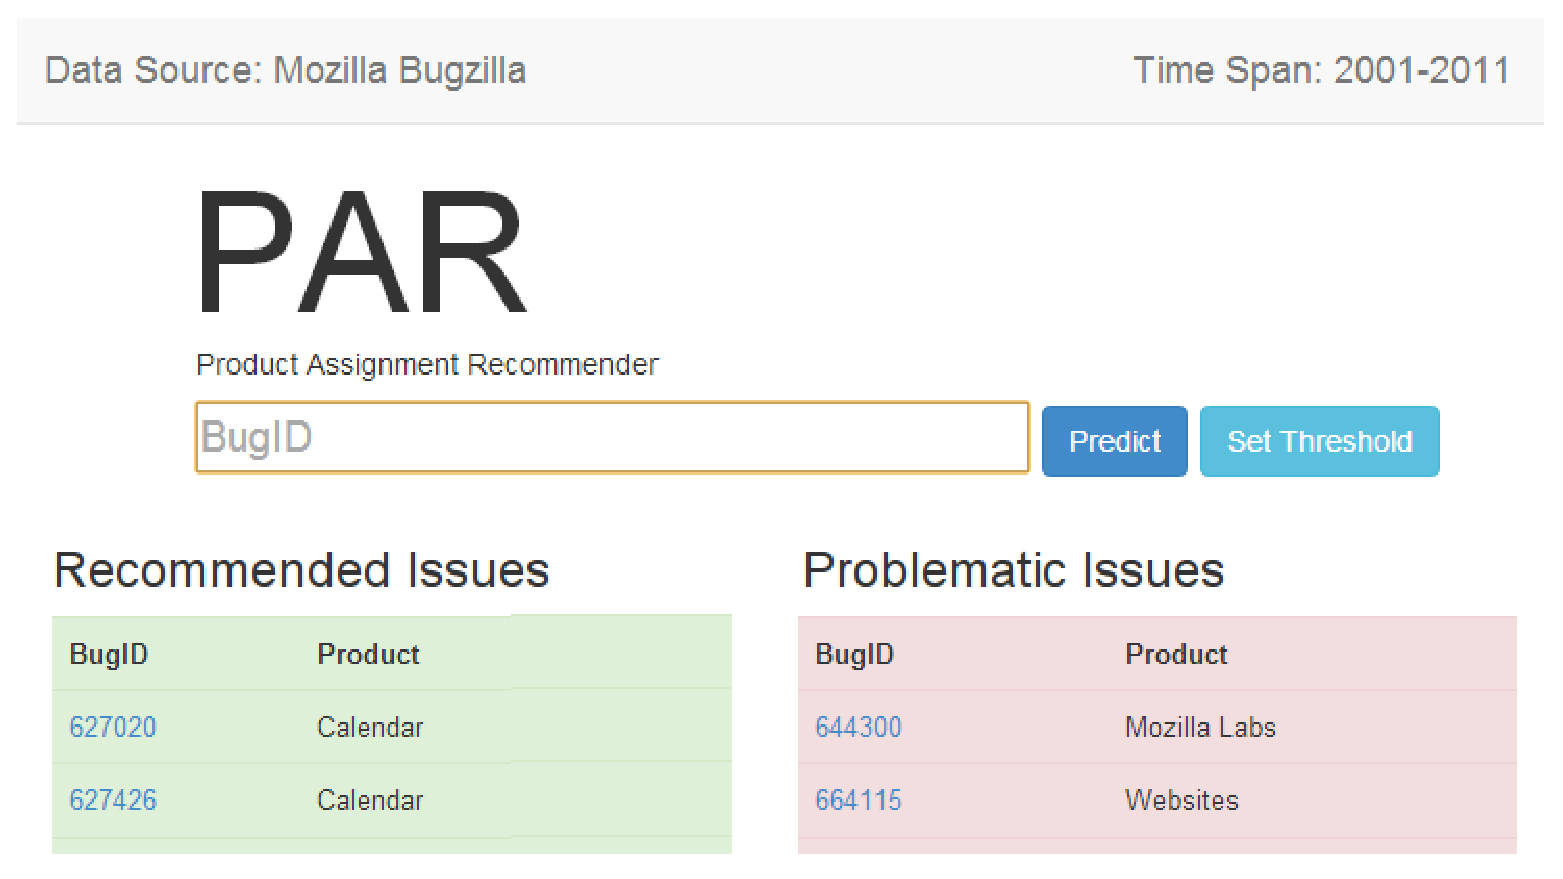
\epsfig{file=query.eps, width=3.1in}
\fbox{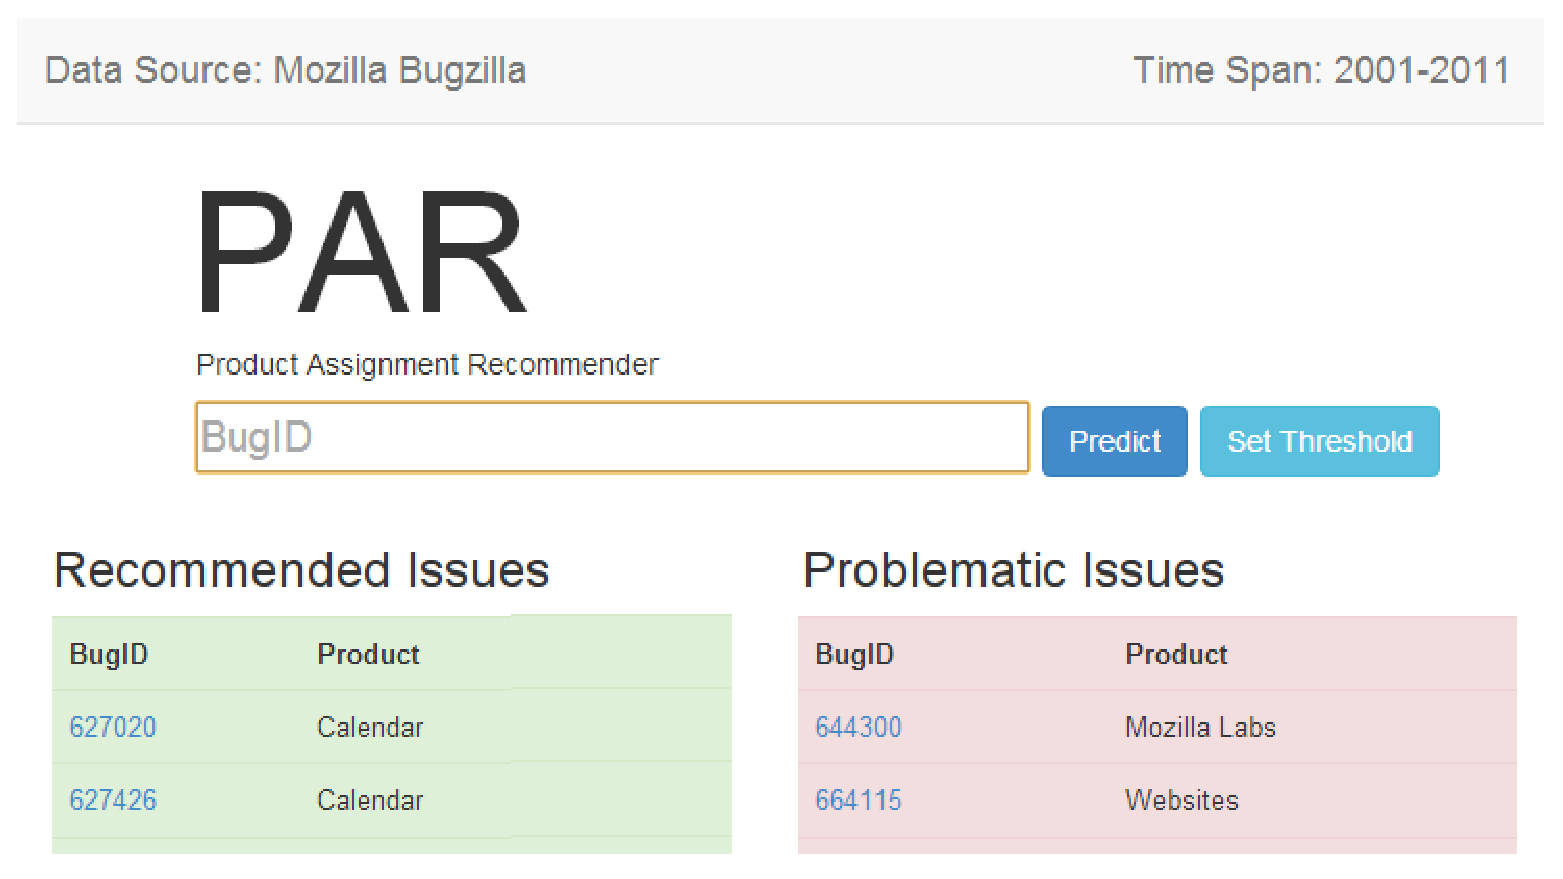
\includegraphics[width=3.1in, height=1.8in]{query.eps}}
\caption{PAR Query Page}\label{fig:query}
\vspace{-.35cm}
\end{figure}

\begin{figure}[ht]
\vspace{-.3cm}
\centering
\fbox{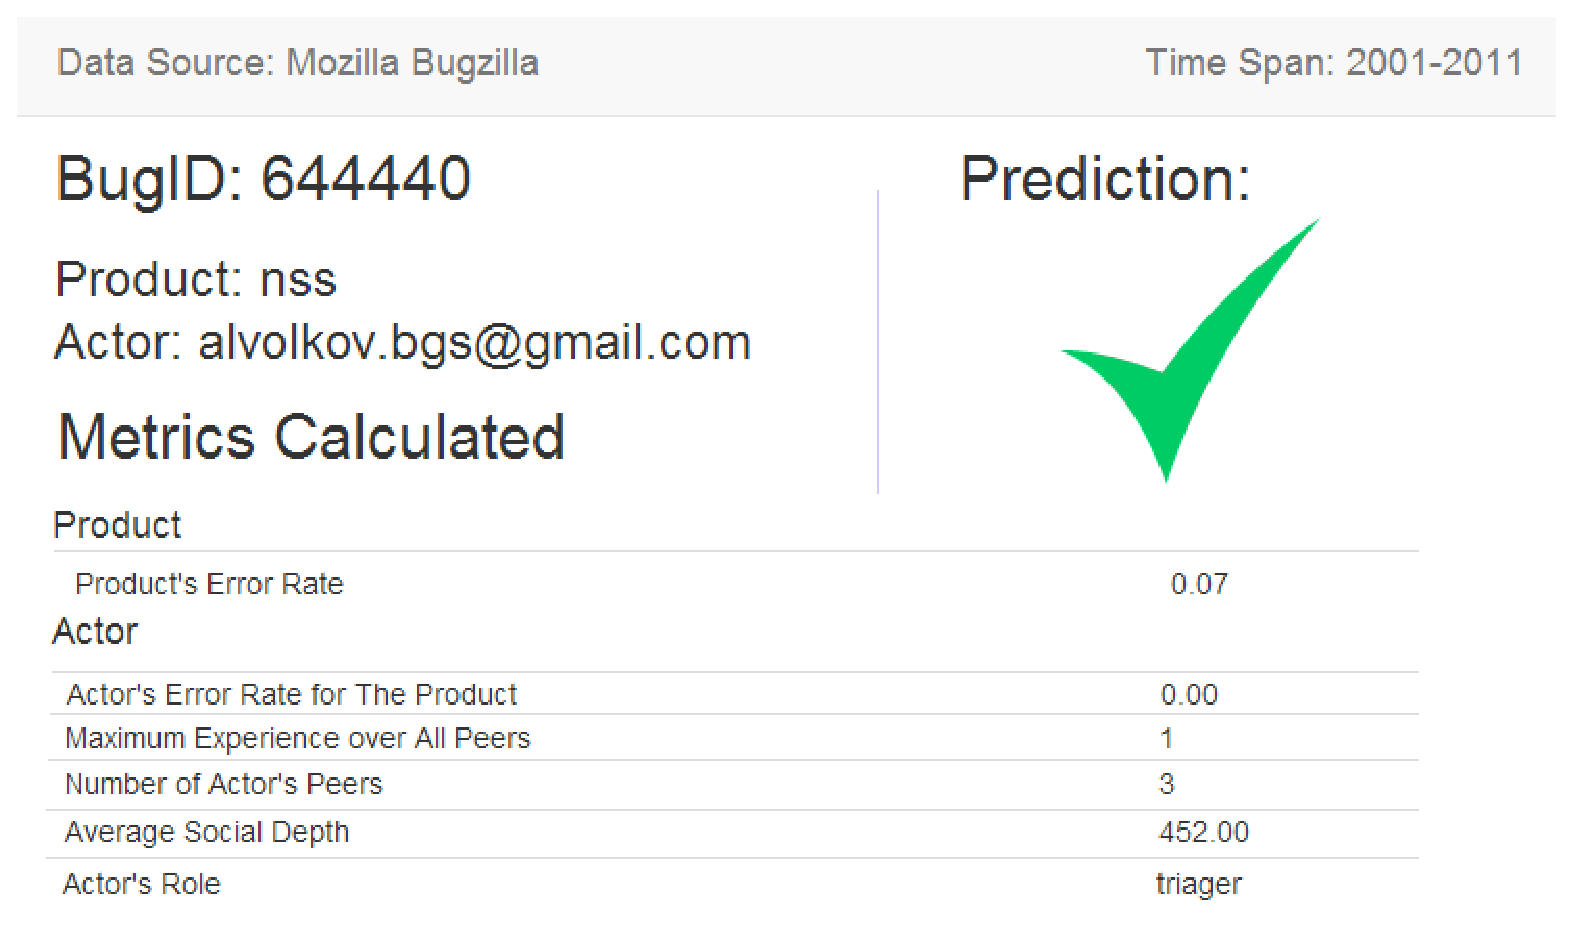
\includegraphics[width=3.1in, height=1.8in]{result.eps}}
\caption{PAR Results Page}\label{fig:result}
\vspace{-.35cm}
\end{figure}


% For demonstration, we implement PAR as an online tool. (Note that it could be
% converted into a plug-in for ITS for practical use.)

We implement PAR with Browser/Server architecture. PAR consists of two parts
-- a backend server that processes data and a web interface
that interacts with the user. In practice, PAR would be the most
effectively used as a plug-in for an ITS.

On the backend, the server extracts recent records from ITS and fits
the model described in Section~\ref{ss:model}.  As requested, PAR
examines the status of the queried issue to see whether it needs
prediction (for example, resolved issues do not need
prediction). After that, the records of the latest product
assignment to the issue, including the assigned product, the login
of the assigner and the time stamp, are extracted, and used to
calculate the measures shown in Table~\ref{tab:predictors}.  PAR
then uses the fitted model coefficients to calculate the predicted
accuracy of the assignment.  Finally, to give a recommendation, PAR
uses two thresholds, $C_r$ and $C_g$ ($C_r < C_g$), to classify the
issues.  If the probability of being correct is below $C_r$, the issue will be
classified as ``Problematic'', suggesting that the assignment should be
verified. If the probability is above $C_g$, the issue will
be classified as ``Recommended'', suggesting that it is ready for
developers. The remaining issues would be classified as ``Not
Recommended''. For a project to take full advantage of PAR, it simply
needs to evaluate incoming issues with PAR and then send them to a
correct queue (typically an email alias).

PAR lists the top-10 ``Recommended'' and
``Problematic'' issues as sketched in Figure~\ref{fig:query}\footnote{Only two issues are shown in the figure to save space}.
A developer
may pick an issue from the ``Recommended'' list
to fix. A triager, on the other hand, would examine issues in the
``Problematic'' list to verify
product assignments. She can also submit a query for
specific issue by typing in the issue ID. Then, in Figure~\ref{fig:result},
the predicted result will be shown together with the measures.

The setting of the thresholds ($C_r$ and $C_g$) requires expertise
and depends on contributor's desired trade-off between precision and
recall. Therefore, PAR provides the opportunity to set the
thresholds by the quantiles of product assignment accuracy. For
example, a busy developer may prefer a high $C_g$,
to ensure that all the issues are for her product. However, she may
miss many correctly assigned issues. Similarly, a triager may prefer
a lower $C_r$ to clean up issues that are most likely to be
incorrectly assigned.

\vspace{-.275cm}
\section{Related work}\label{s:relatedwork}
%There has been a substantial amount of work focusing on different aspects of bug
%reports, such as assisting bug assignment and detecting duplicate bug reports.

Past research has used software repository data to help bug assignment.
For example, Anvik et al.~\cite{Anvik2006} applied a machine learning algorithm to learn
the kinds of reports each developer resolves and recommend developers for
a new report.
Jeong et al.~\cite{Jeong2009} introduced a Markov-chain-based
graph model to recognize bug tossing history.
Xuan et al.~\cite{xuan2012} proposed developer
prioritization to rank the contributions of developers to assist the task of bug triaging.

Detecting duplicate reports is another recurring topic and various methods have
been used to compare the similarity between issue reports. Runeson et al. ~\cite{Runeson07}
investigated using Natural Language Processing (NLP) techniques to identify
duplicate reports. Wang et al.~\cite{Wang2008} used execution information to suggest
the most similar bug reports to the new bug report to the triager.

Foutse K. et al.~\cite{hassan2011} used
entropy and frequency information to detect the crash reports. Weiss et al.~\cite{Weiss07} used
the Lucene framework to search for similar, earlier reports and used their average time
as a prediction for a new report.

To the best of our knowledge, this demo is the first attempt to
predict the accuracy of data in an ITS and to make recommendations
based on that estimate.

\vspace{-.2cm}
\section{Conclusion}\label{s:conclusion}
In this demo, we aim to improve the effectiveness of development
process by predicting the accuracy of data in an ITS
system. In particular, we focus on a problem of product assignment
accuracy because it is often assigned incorrectly in Mozilla and
in commercial projects, and the incorrect assignments lead to
significant delays and wasted effort. A project using our tool
would help developers to focus their limited time on
the relevant issues.

We quantified several aspects of the product and of the assigner
by using issue workflow and modeled how they affect
the probability of an issue being (in)correctly assigned.  Based on
the model, we designed PAR to recommend
issues that are unlikely to waste developers' time,
and to highlight problematic issues that need further
triage to improve the accuracy of product assignment.
Our results on Mozilla Bugzilla dataset show
that the model reaches a precision of 73.65\% or 3.4 times
higher than a random predictor.

We plan to model accuracy of other fields and integrate the model
into PAR.  We also plan to extend PAR in both commercial and open
source projects to improve effectiveness of the development process
by improving quality of data used to direct development work.

\balance
\section{Acknowledgments}
Support by National Basic Research Program of China Grant
2011CB302604 and the National Natural Science Foundation of China
Grants 91118004, 61121063 and 61073016.

%\bibliographystyle{abbrv}
%\bibliography{all,minghui,audirs}  % sigproc.bib is the name of the Bibliography in this case
\vspace{-.22cm}
\begin{thebibliography}{10}

%\bibitem{mztriage}
%Mozilla triage guide -- harnessing the flood of community.
%\newblock \url{https://wiki.mozilla.org/QA/Triage}, 2010.

\bibitem{Anvik2006}
J.~Anvik, L.~Hiew, and G.~C. Murphy.
\newblock Who should fix this bug?
\newblock In ICSE '06, pages 361--370, New York, NY, USA, 2006.

\bibitem{Jeong2009}
G.~Jeong, S.~Kim, and T.~Zimmermann.
\newblock Improving bug triage with bug tossing graphs.
\newblock In ESEC/FSE '09, pages 111--120, New York,
  NY, USA, 2009.

\bibitem{hassan2011}
F.~Khomh, B.~Chan, Y.~Zou, and A.~E. Hassan.
\newblock An entropy evaluation approach for triaging field crashes: A case
  study of Mozilla Firefox.
\newblock {\em Reverse Engineering, Working Conference on}, 0:261--270, 2011.

\bibitem{Changes07}
A.~Mockus.
\newblock Software support tools and experimental work.
\newblock In V.~Basili and et~al, editors, {\em Empirical Software Engineering
  Issues: Critical Assessments and Future Directions}, volume LNCS 4336, pages
  91--99. Springer, 2007.

\bibitem{Runeson07}
P.~Runeson, M.~Alexandersson, and O.~Nyholm.
\newblock Detection of duplicate defect reports using natural language
  processing.
\newblock In ICSE '07, pages 499--510, Washington, DC, USA, 2007.

\bibitem{Wang2008}
X.~Wang, L.~Zhang, T.~Xie, J.~Anvik, and J.~Sun.
\newblock An approach to detecting duplicate bug reports using natural language
  and execution information.
\newblock In ICSE '08, pages 461--470, New York, NY, USA, 2008.

\bibitem{Weiss07}
C.~Weiss, R.~Premraj, T.~Zimmermann, and A.~Zeller.
\newblock How long will it take to fix this bug?
\newblock pages 20--26, May 2007.

\bibitem{XZM13}
J.~Xie, M.~Zhou, and A.~Mockus.
\newblock Impact of triage: a study of mozilla and gnome.
\newblock In {\em ESEM 2013}, pages 247--250, Baltimore, Maryland, USA, Oct
  10--11 2013.

\bibitem{xuan2012}
J.~Xuan, H.~Jiang, Z.~Ren, and W.~Zou.
\newblock Developer prioritization in bug repositories.
\newblock In {\em ICSE 2012}, pages 25 --35, Zurich, Switzerland, June 1--9 2012.

\bibitem{MM12}
M.~Zhou and A.~Mockus.
\newblock What make long term contributors: Willingness and opportunity in open
  source community.
\newblock In {\em ICSE 2012}, pages 518--528, Zurich, Switzerland, June 1--9 2012.

\end{thebibliography}

\end{document}

